\documentclass{article}
\DeclareUnicodeCharacter{0019}{ }
\usepackage[utf8]{inputenc}
%\usepackage{mathabx}
%\usepackage{amsopn}
\usepackage{cite}
\usepackage{graphicx}
\usepackage{float}
\usepackage{caption}
\usepackage{amsmath}
\setlength\parindent{0pt}
\graphicspath{{C:\Users\Pruthvi\git\phmehta95\thesis\thesis}}
\usepackage{chemformula}



\title{Systematic uncertainty calculations}

\begin{document}
\maketitle



\section{Systematic uncertainty calculation methodology}\label{systmethod}


The systematic uncertainities for this analysis are calculated using the probablity distribution functions of each quantity appearing in the formula for the mean neutron multiplicity, which is given by:

\begin{equation}
    M=\frac{\# n_{\text {det }}-R \times \# \nu_{\text {det }}}{T} \frac{1}{\# \nu_{\text {det }}}
 \label{multiplicity}
\end{equation}



By random sampling the probability distribution functions for each of the terms in Equation \eqref{multiplicity} one can calculate the multiplicity probability distribution functions for both the statistical uncertainty and the systematic uncertainty. The statistical uncertainty for the value for the multiplicity is related to the variation in the number of detected neutrons, while the systematic uncertainty is related to the variation on the tagging efficiency and the background rate. The total search time for the tagged neutrons is dependent on the number of "windows" in which the neutron is searched for in, and therefore the term for the number of detected neutrinos. Because any variation on the number of neutrinos which are detected is unrelated to the value for the mean neutron multiplicity, calculating a probability mass function for the number of neutrinos is uneccessary. 

A Poissonian distribution is used to model the distribution for the number of detected neutrons, due to its value being approximated by counting the positives in the timing window that the neutron tagging search is carried out in. The mean value of this Poisson distribution is denoted in Equation \eqref{poissonuncertainty}.
\newline
\begin{equation}
    P M F\left(\# n_{\text {det }}\right)=\frac{1}{\left(\# n_{\text {det }}\right) !}\left\langle \# n_{\text {det }}\right\rangle^{\# n_{\text {det }}} e^{-\left\langle \# n_{\text {det }}\right\rangle}
\label{poissonuncertainty}
\end{equation}
\newline
Regarding the background rate, this is estimated from dummy spill data, but it's error is associated with the statistical variation of the Monte Carlo size that the backround rate is associated with, and secondly the change of the background rate value during the SK-V period. The statistical variation of the MC is modelled using a Gaussian, while the uncertainty relating to time variation is characterised by its own probability distribution function. In contrast, the tagging efficiency is model dependent and has systematic uncertainties relating to this. The two ways in which the systematic error are estimated are either using MC re-weighting or MC regeneration.
\newline
For the MC-reweighting approach, weights are applied to a quantity and the tagging efficiency of the re-weighted MC is extracted. The general methodology is to have the input of a model (given by a set of parameters) and to vary them one by one and then calculate the reweighted tagging efficiencies - the set of relative discrepancies $\delta_{i}$ are computed from this set of reweighted tagging efficiencies $T_{i}$ and the nominal tagging efficiency $T_{nom}$ using Equation \eqref{tageffdiscrep}.
\newline
\begin{equation}
    \delta_{i}=\frac{T_{i}-T_{\text {nom }}}{T_{\text {nom }}} \quad i \in\{\text { parameters }\}
\label{tageffdiscrep}
\end{equation}
\newline

These relative discrepancies $\delta_{i}$ are used to calculate the one indivdual discrepancy $\delta_{reweighted}$ that would describe the final deviation from the nominal tagging efficiency $T_{nom}$ due to the systematic error. $\delta_{reweighted}$ describes the model which has been produced through 1$\sigma$ variations of these parameters, therefore the final probability distribution function which describes the deviation from the nominal MC has a Gaussian distribution with the standard deviation being equal to $\delta_{reweighted}$. 
\newline
The other method to estimate the systematic error on the tagging efficiency is the method of Monte Carlo regeneration. This is carried out by varying a parameter then regenerating the whole Monte Carlo and then extracting the tagging efficiency - therefore unlike with MC re-weighting there is no set of discrepancies $\delta_{i}$ but instead two single discrepancies $\delta_{min}$ and $\delta_{max}$. The resulting probability distribution which describes the deviation from the nominal Monte Carlo is a Gaussian which has the mean and standard deviation relating to the discrepancies shown in Equation \eqref{mcregengauss}.
\newline

\begin{equation}
\left\{\begin{array}{l}
\mu=\frac{\delta_{\max }+\delta_{\min }}{2} \\
\sigma=\frac{\delta_{\max }-\delta_{\min }}{2}
\end{array}\right.
\label{mcregengauss}
\end{equation}


\section{Neutrino beam flux uncertainty}

The uncertainty on neutrino beam fluxes can also be evaluated by looking at the dependence of the tagging efficiency on the flux variations. The beam fluxes for the four flavour modes 
$\left(\nu_{e} \overline{\nu_{e}} \nu_{\mu} \overline{\nu_{\mu}}\right)$ have the fractional uncertainties given for each mode, FHC and RHC. The binned uncertainties are shown in Figure .


Each individual bin for the flux is increased/decreased by its error, the Monte Carlo re-weighting method is then used to extract the taggging efficiency for each flux bin, and Equation \eqref{nubeamfluxerror} is used to calculate the fractional uncertainty.
\newline
\begin{equation}
    \delta_{i}(\pm \sigma)=\frac{T_{i}(\pm \sigma)-T_{\text {nom }}}{T_{\text {nom }}} \quad i \in\{\text { each flux bin }\}
\label{nubeamfluxerror}
\end{equation}
\newline
Figure \ref{fig:fluxuncertainty} shows the fractional errors calculated from the reweighted Monte Carlo, with the red bars showing the -1$\sigma$ variation and the blue bars showing the +1$\sigma$ variation. Table \ref{table:systuncertaintytable} contains the value for the total fractional uncertainty resulting from the neutrino beam flux, which was calculated using Equation \eqref{summingfluxuncertainty}, where the maximum value between the increased and decreased discrepancy is taken and summed over to produce the final neutrino flux beam uncertainty value.
\newline

\begin{equation}
    \delta_{\nu \text { flux }}=\sum_{i \in\{\text { bins }\}} \max \left[\left|\delta_{i}(+\sigma)\right|,\left|\delta_{i}(-\sigma)\right|\right]
 \label{summingfluxuncertainty}   
\end{equation}

\begin{figure}[h!]
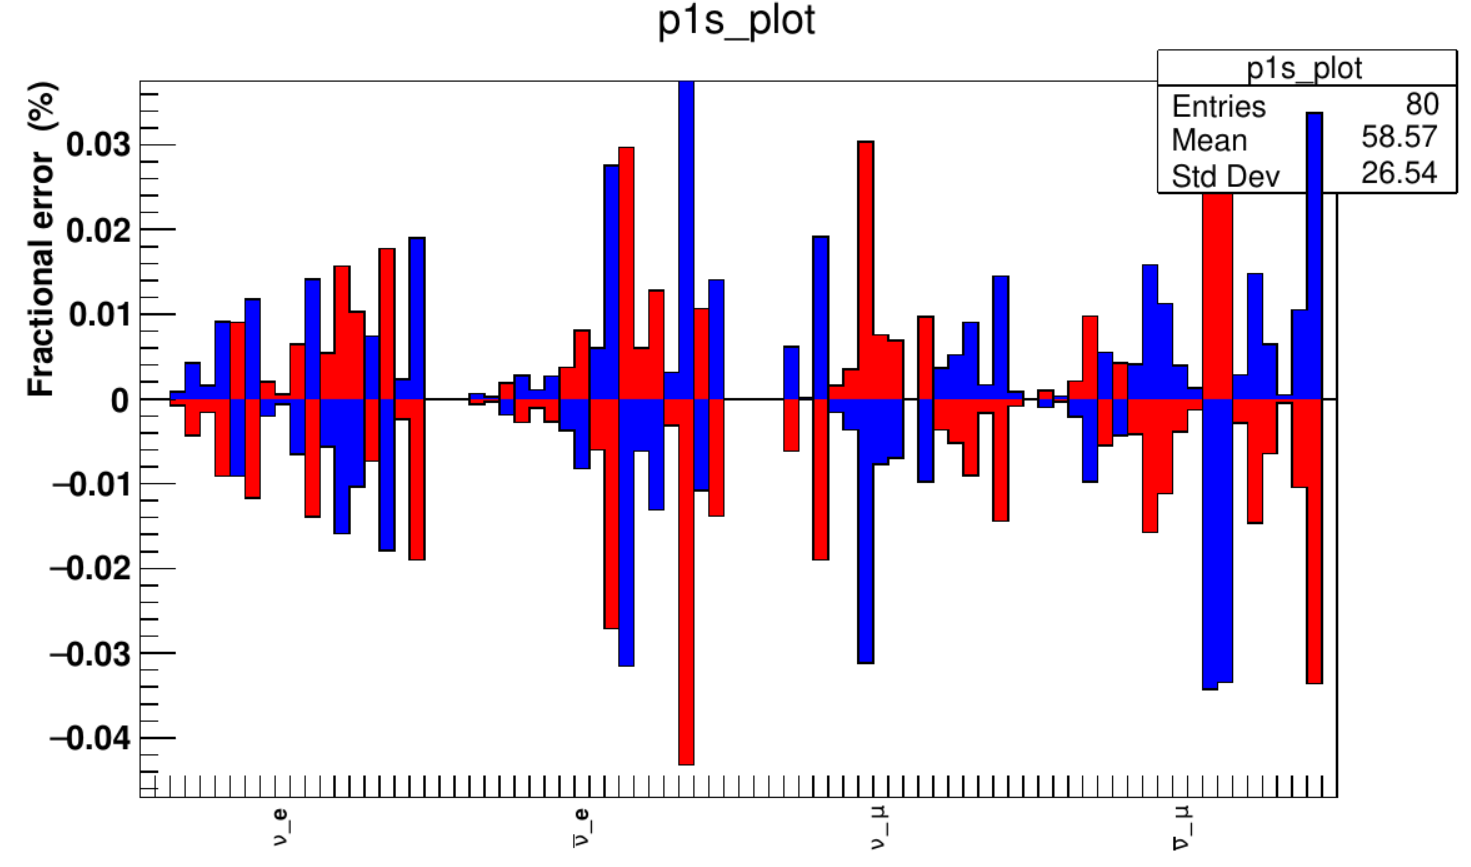
\includegraphics[scale=0.4]{flux_uncertainty.png}
\caption{Tagging efficiency fractional uncertainties caused by neutrino beam flux discrepancies. From left to right the sections in this plot are comprised of the beam fluxes elements of $\left(\nu_{e} \overline{\nu_{e}} \nu_{\mu} \overline{\nu_{\mu}}\right)$ respectively.}
\label{fig:fluxuncertainty}
\end{figure}

\section{Neutrino cross section uncertainty}

A group of default neutrino cross section values are used to make up the nominal Monte Carlo from which the tagging efficiency is calculated. The values of the parameters that determine the cross sections are shown in Table \ref{xsectable}. Each of the parameter values relate to a specific interaction type and are either a normalisation parameter or a paramater which show a kinematic dependence. The re-weighting method mentioned in Section \ref{systmethod} is used to reweight the nominal Monte Carlo on an event by event basis with each parameter value being increased and decreased by its uncertainty, and for each reweighted Monte Carlo the equivalent tagging efficiency value is extracted. Equation \eqref{xsectageff} shows how the fractional discrepancies are extracted from the nominal and reweighted tagging efficiency values.

\begin{equation}
\delta_{i}(\pm \sigma)=\frac{T_{i}(\pm \sigma)-T_{\text {nom }}}{T_{\text {nom }}} \quad i \in\{\text { parameters }\}
\label{xsectageff}
\end{equation}

Figure \ref{fig:xsecuncertainty} shows the reweighted Monte Carlo fractional uncertainty plotted for the FHC sample. Since this sample contains a lot of NCother interactions, the uncertainty for this interaction type is greater than for the others.

\begin{table}
$$
\begin{array}{llll}
\hline & & & \\
\text { Parameter } & \text { Interaction } & \text { Type } & \text { Value } \\
& & & \\
p_{F}^{O} & \mathrm{CCQE} & { }^{16} \mathrm{O} \text { Fermi momentum } & 225 \pm 31 \mathrm{MeV} / \mathrm{c} \\
E_{B}^{O} & \mathrm{CCQE} & { }^{16} \mathrm{O} \text { binding energy } & 27 \pm 9 \mathrm{MeV} \\
M_{A}^{C C Q E} & \mathrm{CCQE} & \text { Axial mass } & 1.2 \pm 0.41 \mathrm{GeV} / \mathrm{c}^{2} \\
2 p 2 h & & & \\
C_{A S}^{R E S} & 2 \mathrm{p} 2 \mathrm{~h} & \text { Normalization par. } & 1.0 \pm 1.0 \\
M_{A}^{R E S} & \mathrm{CC} \text { and } \mathrm{NC} 1 \pi & \text { Axial form factor } & 1.01 \pm 0.12 \\
B G_{A}^{R E S} & \mathrm{CC} \text { and NC1 } \pi & \text { Axial mass } & 0.95 \pm 0.15 \mathrm{GeV} / \mathrm{c}^{2} \\
\mathrm{CC} \text { other } & \mathrm{CC} \text { and } \mathrm{NC} 1 \pi & \mathrm{I}=1 / 2 \text { continuum background } & 1.3 \pm 0.2 \\
\mathrm{CC} \text { coherent } & \mathrm{CC} \text { other } & \text { E-dependent par. } & 0.0 \pm 0.4 \\
\mathrm{NC} \text { other } & \mathrm{CC} \text { coherent } & \text { Normalization par. } & 1.0 \pm 0.3 \\
\mathrm{NC} \text { coherent } & \mathrm{NC} \text { other } & \text { NC-dependent par. } & 1.0 \pm 0.3 \\
& & \text { Normalization par. } & 1.0 \pm 0.3 \\
\mathrm{FS} e^{-} \text {Bremsstrahlung } & \mathrm{CC} \nu_{e} & \text { Normalization par. } & 1.00 \pm 0.03 \\
\hline
\end{array}
\label{xsectable}
$$
\caption{Neutrino cross section parameters}
\end{table}


\begin{figure}[h!]
    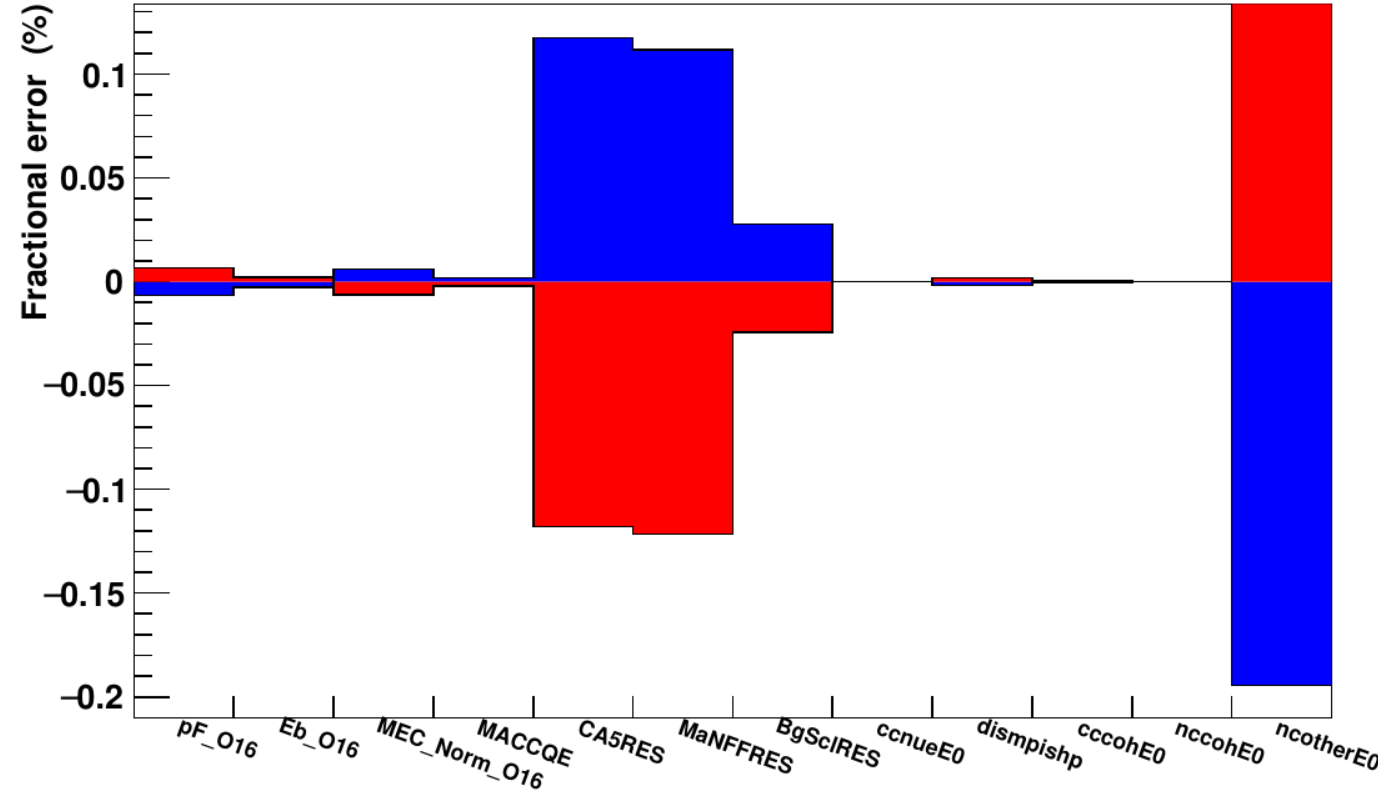
\includegraphics[scale=0.4]{xsec_uncertainty.png}
\caption{Tagging efficiency fractional uncertainty caused by the cross-section parameters variations for the FHC mode}
\label{fig:xsecuncertainty}
\end{figure}

\section{Pion final state interaction (FSI) and secondary interaction (SI) uncertainties}

The neutrino-nucleus interaction simulator used in this analysis (NEUT) handles pion final state interactions and secondary interactions using a cascade model. This cascade model contains parameters which will have uncertainties on them and these will be tranferred to a possible change in the tagging efficiency.

Depending on the momentum of the pions, different interaction types occur in the model. For pions with a momentum less than 500 MeV, the interactions in place are absorption (ABS), quasi-elastic scattering (QE) and charge exchange (CX)./cite{} Absorption occurs when the incident pion is absorbed by the nucleus and no pions remain in the final state. Quasi-elastic (QE) scattering occurs when there is only one pion observed in the final state and it has the same charge as the incident beam. Charge exchange occurs when the charged pion interacts wtht he nucleus and a single $\pi_{0}$ can be seen in the final state.


For pions with a momentum of greater than 500 MeV, a different set of interactions are used. Inelastic interactions (INEL) can now produce hadrons and replace absorption processes, but quasi-elastic scattering (QEH) and charge exchange (CXH) will still occur. The final state interaction parameters and the pion momentum range they are used in can be seen in Table \ref{fsiparameters}. Each parameter scales the relevant very small proabability of the charged pion interaction at every stage of the intra-nuclear cascade, aside from the parameter for charge exchange which scales only the fraction of low momentum QE scattering. 


\begin{table}
$$
\begin{array}{ccc}
\hline \text { Parameter } & \text { Description } & \begin{array}{c}
\text { Momentum } \\
\text { Region }(\mathrm{MeV} / c)
\end{array} \\
\hline f_{\mathrm{ABS}} & \text { Absorption } & <500 \\
f_{\mathrm{QE}} & \text { Quasi-elastic scatter } & <500 \\
f_{\mathrm{CX}} & \text { Single charge exchange } & <500 \\
f_{\mathrm{QEH}} & \text { Quasi-elastic scatter } & >500 \\
f_{\mathrm{CXH}} & \text { Single charge exchange } & >500 \\
f_{\mathrm{INEL}} & \text { Hadron }(\mathrm{N}+\mathrm{n} \pi) \text { production } & >500 \\
\hline
\end{array}
$$
\caption{Table showing the pion final state interaction parameters in NEUT and the pion momentum range they are used in}
\end{table}
A set of paramater variations which determine a surface in paramater space have been estimated by pion scattering experiments, the values for which are shown in Table \ref{fsimodelparameters}. The 1$\sigma$ surface has been explored using the nominal Monte Carlo re-weighting method and the analagous tagging efficiency uncertainty is shown in Equation \ref{fsisitageff}, and the uncertainty stemming from the models shown in Table \ref{fsimodelparameters} is shown in Figure \ref{fig:fsisiuncertainty}

\begin{equation}
\delta_{i}=\frac{T_{i}-T_{\text {nom }}}{T_{\text {nom }}} \quad i \in \text { parameter vector }
\label{fsisitageff}
\end{equation}

\begin{figure}[h!]
    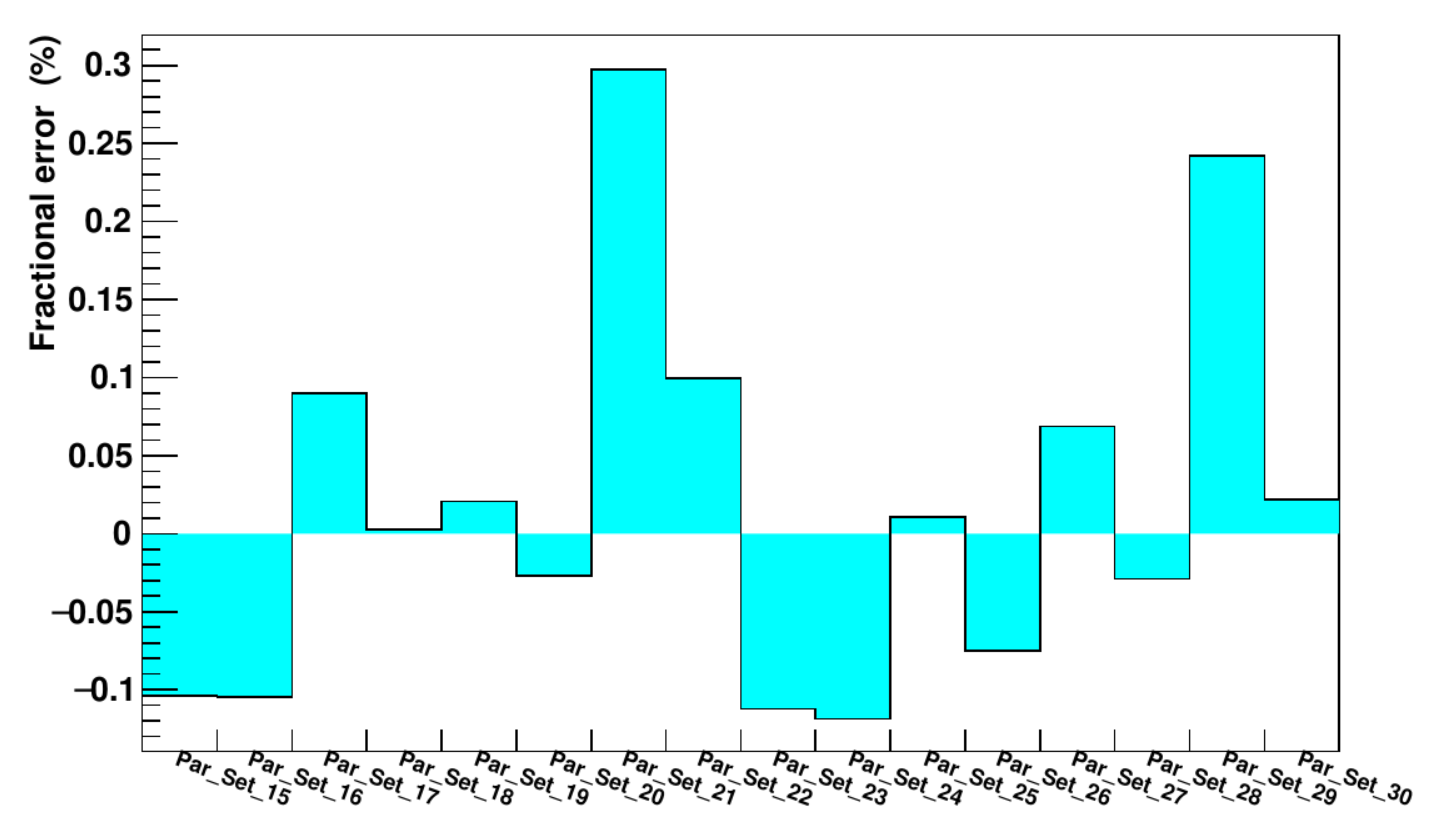
\includegraphics[scale=0.4]{fsisi_uncertainty.png}
\caption{Tagging efficiency fractional uncertainty caused by the variation in the FSI/SI model parameters for the FHC mode.}
\label{fig:fsisiuncertainty}
\end{figure}

\begin{table}
    $$
    \begin{array}{lllllll}
        \hline & & & & & & \\
        \text { Set } & \text { ABS } & \text { QE } & \text { CX } & \text { INEL } & \text { QEH } & \text { CXH } \\
        \hline
    %\begin{array}{ccccccc}
    \text { Nominal } & 1.1 & 1.0 & 1.0 & 1.0 & 1.8 & 1.8 \\
    & & & & & & \\
    & 0.7 & 0.6 & 0.5 & 1.5 & 1.1 & 2.3 \\
    & 0.7 & 0.6 & 1.6 & 1.5 & 1.1 & 2.3 \\
    \text { Hadron production Up } & 1.6 & 0.7 & 0.4 & 1.5 & 1.1 & 2.3 \\
    & 1.6 & 0.7 & 1.6 & 1.5 & 1.1 & 2.3 \\
    & 0.6 & 1.4 & 0.6 & 1.5 & 1.1 & 2.3 \\
    & 0.7 & 1.3 & 1.6 & 1.5 & 1.1 & 2.3 \\
    & 1.5 & 1.5 & 0.4 & 1.5 & 1.1 & 2.3 \\
    & 1.6 & 1.6 & 1.6 & 1.5 & 1.1 & 2.3 \\
    & & & & & & \\
    & 0.7 & 0.6 & 0.5 & 0.5 & 2.3 & 1.3 \\
    & 0.7 & 0.6 & 1.6 & 0.5 & 2.3 & 1.3 \\
    & 1.6 & 0.7 & 0.4 & 0.5 & 2.3 & 1.3 \\
    \text { Hadron production Down } & 1.6 & 0.7 & 1.6 & 0.5 & 2.3 & 1.3 \\
    & 0.6 & 1.4 & 0.6 & 0.5 & 2.3 & 1.3 \\
    & 0.7 & 1.3 & 1.6 & 0.5 & 2.3 & 1.3 \\
    & 1.5 & 1.5 & 0.4 & 0.5 & 2.3 & 1.3 \\
    & 1.6 & 1.6 & 1.6 & 0.5 & 2.3 & 1.3
    \end{array}
    $$
\caption{Pion FSI/SI model parameter nominal value and variations grouped according to inelastic hadron production value}
\end{table}

\section{Nucleon final state interactions}

Uncertainties regarding the nucleon final state interactions can change the number of nucleons knocked out of 16O, therefore how the tagging efficiency is changed due to the variation in nucleon final state interactions needs to be investigated. This uncertainty is extracted using GENIE, a Monte Carlo event generator which contains the INTRANUKE (hA) intranuclear transport model. The uncertainties in the in the total scattering probability for hadrons inside the target nuclei ($x_{m f p}^{N}$) and the uncertainties in the likelihood of each hadron rescattering method: (elastic ($x_{e l}^{N}$), inelastic ($x_{i n e l}^{N}$), charge exchange ($x_{c e x}^{N}$), pion production ($x_{\pi}^{N}$) and absorption ($x_{a b s}^{N}$)) are taken into account. The fractional uncertainties for these modes for pions is shown in Table \ref{nucleonfsiuncertainties}. 

\begin{table}
$$
\begin{array}{llc}
\hline \text {Abbreviation} & \text { Description of uncertainty }  & \text{Fractional uncertainty} \\
\hline x_{m f p}^{N} & \text { Nucleon mean free path (total rescattering probability) } & \pm 20 \% \\
x_{c e x}^{N} & \text { Nucleon charge exchange probability } & \pm 50 \% \\
x_{e l}^{N} & \text { Nucleon elastic reaction probability } & \pm 30 \% \\
x_{i n e l}^{N} & \text { Nucleon inelastic reaction probability } & \pm 40 \% \\
x_{a b s}^{N} & \text { Nucleon absorption probability } & \pm 20 \% \\
x_{\pi}^{N} & \text { Nucleon } \pi \text {-production probability } & \pm 20 \%
\end{array}
$$
\caption{Nucleon final state interaction parameters of the hA model executed inside GENIE.} 
\label{nucleonfsiuncertainties}
\end{table}

A nominal GENIE Monte Carlo sample is generated (different from the previously used NEUT Monte Carlo) and this shifted using the re-weighting method to a varied GENIE Monte Carlo by individually increasing and decreasing the parameters in Table \ref{nucleonfsiuncertainties} by its error. For each shifted Monte Carlo produced, the fractional uncertainty can be written as in Equation \ref{nucleonfsitageff}.

\begin{equation}
\delta_{i}(\pm \sigma)=\frac{T_{i}(\pm \sigma)-T_{\text {nom }}}{T_{\text {nom }}} \quad i \in\{\text { parameters }\}
\label{nucleonfsitageff}
\end{equation}

The tagging efficiency fractional uncertainties are displayed in Figure \ref{fig:nucleonfsiuncertainty}, showing which parameter from Table \ref{nucleonfsiuncertainties} each uncertainty has arisen from.

\begin{figure}[h!]
    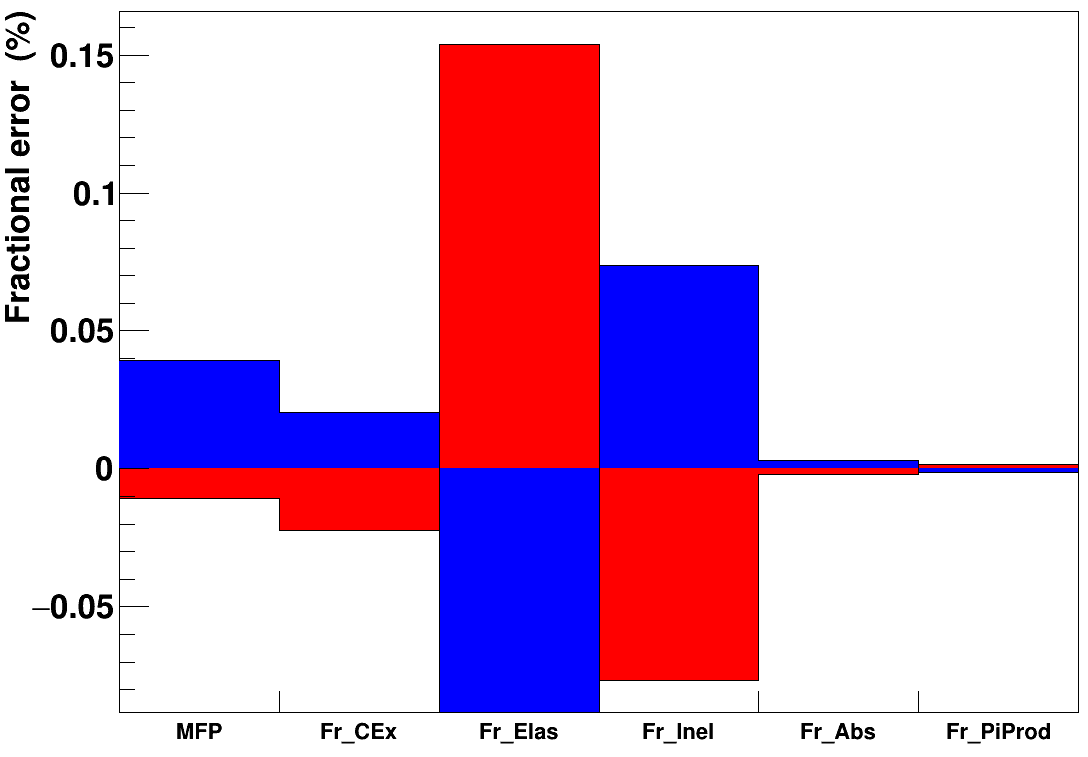
\includegraphics[scale=0.4]{nucleonfsi_uncertainty.png}
\caption{Tagging efficiency fractional uncertainties caused by the nucleon final state interaction model parameter variation for the FHC mode}
\label{fig:nucleonfsiuncertainty}
\end{figure}




\end{document}